\documentclass[11pt]{article}
\usepackage[utf8]{inputenc}
\usepackage{amsmath}
\usepackage{amsfonts}
\usepackage[margin=1in]{geometry}
\usepackage{framed}
\usepackage{tikz}
\usepackage{listings}
\usepackage{graphicx}
\usepackage{bbm}
\usepackage{amsthm}
\newtheorem{theorem}{Theorem}
\newtheorem{corollary}{Corollary}[theorem]
\newtheorem{lemma}{Lemma}[theorem]
\newtheorem{assumption}{Assumption}[theorem]
\newtheorem*{remark}{Remark}
\usepackage{amssymb}
\usepackage{mathrsfs}
\usepackage{amsthm}

\usepackage{mathtools}
%\pagenumbering{gobble}
\newcommand{\maxl}{\lambda}
\newcommand{\vlen}{\boldsymbol{h}}
\newcommand{\vint}{\boldsymbol{\omega}}
\newcommand{\vpla}{\boldsymbol{a}}
\newcommand{\innerone}{D_{11}}
\newcommand{\inneronej}{D_{11j}}
\newcommand{\innertwo}{D_{12}}
\newcommand{\innertwoj}{D_{12j}} 
\newcommand{\innerthree}{D_{22}}
\newcommand{\biasone}{B_1}
\newcommand{\biastwo}{B_2}
\newcommand{\biasthree}{B_3}
\newcommand{\Imn}{D}
\newcommand{\Tmn}{T}
\newcommand{\io}{\mathscr{Q}_{p,q}}
\newcommand{\slle}{\hat{\mu}^{LL}_{0j}}
\linespread{1}
\usepackage{bbold}
\usepackage[utf8]{inputenc}
\usepackage{dirtytalk}
\usepackage{float}

\newcommand{\bigCI}{\mathrel{\text{\scalebox{1.07}{$\perp\mkern-10mu\perp$}}}}
%\usepackage{cite}
%\usepackage[backend=bibtex,style=verbose-trad2]{biblatex}
%\bibliography{lesson7a1} 
%\bibliographystyle{ieeetr}

\DeclareMathOperator*{\argmin}{arg\,min}
\DeclareUnicodeCharacter{2014}{\dash}
\usepackage{hyperref}
%\usepackage{natbib}
\usepackage{url}

\usepackage[numbers]{natbib}
\bibliographystyle{plainnat} 

%\usepackage{biblatex}
%\addbibresource{prelim.bib}

%\bibliographystyle{plain}

%\DeclareUnicodeCharacter{0027}{\dash}
%\DeclareRobustCommand\dash{%
%  \unskip\nobreak\thinspace\textemdash\allowbreak\thinspace\ignorespaces}
%\bibliography{prelim} 
%\pagestyle{headings}
\allowdisplaybreaks
\newcommand{\Var}{\textrm{Var}}
\newcommand{\Cov}{\textrm{Cov}}
\newcommand{\Br}{\mathcal{B}(\mathbb{R})}

 \title{Teaching Statement}
 \author{}
% %\date{Committee Members: Tailen Hsing, Kerby Shedden, Stilian Stoev}
% \date{April 24, 2019}

\begin{document}



%We propose the model \begin{align*}
%C(s_1, p_1, s_2, p_2) &= \sum_{k=1}^K Y_k(
%\end{align*}

%\section{Functional Setup}
%
%We consider the Argo data residuals $\{ \{p_{i,j}, T_{i,j}\}_{j=1}^{m_i}, t_i, s_i\}_{i=1}^N$ where $i$ denotes the profile and $j$ denotes an individual measurement. For now, we take $T_{i,j}$ to be temperature and $\mathbb{E}(T_{i,j}) = 0$ for all $i$ and $j$. For now, we ignore the times $t_i$.
%
%Tailen has suggested the model \begin{align}
%T_{i,j} &= \sum_{k=1}^K Y_{k}(s_i) \phi_k(p_{i,j})\label{funmodel}
%\end{align}for some small $K$. The $Y_{k}(\cdot)$ may have different distributions across $k$ and be dependent across both $s_i$ and $k$. Here, we assume that each $\phi_k$ is a fixed function that has been estimated through some form of functional principal component analysis (FPCA). 
%
%Let $T^*(p)$ and $Y^*(s_0) \in \mathbb{R}^K$ be the respective predictions at a fixed location $s_0$, and $Y$ to denote all $Y_k(s_i)$ in a radius of $s_0$ from three consecutive months of the year. Let $n$ be the number of profiles in this radius. From here, one can see that \begin{align*}
%\mathbb{E}(T^*(p) |  Y) &= \sum_{k=1}^K \mathbb{E}(Y^*_k(s_0) | Y) \phi_k(p) 
%\end{align*}
%by linearity of expectation and 
%\begin{align*}
%\Var(T^*(p) |  Y) &=\Var\left( \sum_{k=1}^K Y^*_k(s_0) \phi_k(p) \bigg| Y\right) \\
%&= \sum_{k=1}^K \phi_k(p)^2 \Var(Y_k^*(s_0) | Y) + 2\sum_{k\neq \ell} \phi_k(p)\phi_{\ell}(p)\Cov(Y_k^*(s_0),  Y_\ell^*(s_0) | Y).
%\end{align*}
%Assuming that the field of $\{Y_{k}(s_i)\}_{i=1, k=1}^{n, K}$ is jointly multivariate normal and the $T_{i,j}$ follow model (\ref{funmodel}), then the conditional mean and variance completely describe the predictive distribution of $T^*(p)$, since it is a linear combination of $Y^*$. 
%
%%Consider a multivariate spatial model fixed, and let $\{Y_{k}(s_i)\}_{i=1, k=1}^{n, K}$ be data near a fixed location $s_0$ and in the first three months of the year. 
%Suppose that one has a model for $Y$ and let
%\begin{align*}
%\Sigma_Y &= \Var(Y) \in \mathbb{R}^{nK \times nK}\\
%\Sigma^* &=\Var(Y^*(s_0)) \in \mathbb{R}^{K\times K}\\
%\Sigma_{21} &=\Cov(Y, Y^*(s_0)) \in \mathbb{R}^{nK\times K}
%\end{align*}
%%Let $C_Y = \Var(Y) \in$ be the covariance matrix of the $\{Y_{i,k}\}_{i=1, k=1}^{n, K}$ and $C^* \in \mathbb{R}^K \times K}$ be $\Var(Y^*)$, and $C_{12} = \Cov(Y, Y^*) \in \mathbb{R}\ti
%%
%%Let \begin{align*}
%%C_Y &= \begin{align*}
%%\end{align*}
%Then the conditional expectation is
%\begin{align*}
%\mathbb{E}(Y^*(s_0) | Y) &= \Sigma_{21}^\top \Sigma_Y^{-1} Y
%\end{align*}and the conditional variance is \begin{align*}
%\Var(Y^*(s_0) | Y) &= \Sigma^* - \Sigma_{12}^\top \Sigma_Y^{-1} \Sigma_{12}, 
%\end{align*}which then gives \begin{align*}
%T^*(p) | Y \sim N\left( (\Sigma_{21}^\top \Sigma_Y^{-1} Y)^\top \phi(p),  \ \phi(p)^\top ( \Sigma^* - \Sigma_{12}^\top \Sigma_Y^{-1} \Sigma_{12}) \phi(p) \right)
%\end{align*} where $\phi(p) = \begin{pmatrix} \phi_1(p) & \phi_2(p) & \dots & \phi_K(p)\end{pmatrix}^\top$. 
%



%This gives us a functional covariance of 
%\begin{align*}
%\mathbb{E}(T_{1,1} T_{2,2}) = C(s_1, s_2; p_1, p_2) &= \sum_{k=1}^K \sum_{\ell = 1}^K \mathbb{E}(Y_{1,k} Y_{2,\ell}) \phi_k(p_{1}) \phi_{\ell}(p_2).
%\end{align*}This suggests that we can model the covariance $\Cov(Y_k, Y_\ell)$ to model the entire functional covariance. This requires a multivariate spatial model. 


\section{Multivariate Model for scores}

Given a model for $Y$, the above gives a relevant functional model. We consider the problem here on how to model the scores $Y$. 

%We consider the spatial model where we observe $Y(s_i)$ for $i=1, \dots, n$, $s_i \in \mathbb{R}^d$, and $Y(s_i) \in \mathbb{R}^k$. We might take $k=3$ for now. 

Following Stilian?s formulation, when $d=1$ and $s$ and $t$ are scalar, we consider \begin{align*}
Y(t) &= \int_\mathbb{R}e^{itx}((1 + ix)^{-\nu - 1/2} A1_{\{x > 0\}} + (1 + ix)^{-\nu - 1/2} \overline{A}1_{\{x < 0\}}\tilde{B} (dx)
\end{align*}where $\tilde{B}(dx)$ is $\mathbb{C}^k$-valued Brownian motion with \begin{align*}
\tilde{B}(x) &= \overline{\tilde{B}(-x)} &  \mathbb{E}[\tilde{B}(dx) \tilde{B}(dx)^*] &= \mathbb{I}_k dx
\end{align*}and $A$ is a complex-valued matrix. When $\nu = \nu \mathbb{I}_k$ is a scalar, this above integral gives the covariance \begin{align*}
\mathbb{E}[ Y(t) Y(s)^\top ] &= \int_{\mathbb{R}} e^{i(s-t)x}(1+x^2)^{-\nu-1/2}(AA^*1_{\{x >0\}} + \overline{AA}^*1_{\{x < 0\}})dx.
\end{align*}
%We call this the multivariate Matern model. When $AA^*$ is real, the model is reversible and reduces to a special case of the Gneiting et al (2010) model where each auto-covariance and cross-covariance are Matern.
%
%Computing the integral gives for each component product gives \begin{align*}
%\mathbb{E}[ Y_i(t) Y_j(s) ]  &= \textrm{Re}(z_{i,j}) M( s-t, \nu) + \textrm{Im}(z_{i,j})S\left(s-t , \nu\right).
%\end{align*}where $z_{i,j} = e_i^\top AA^*e_j$ where $\{e_j\}_{j=1}^K$ are the standard basis vectors,  \begin{align*}
%M(h, \nu) &= \frac{\pi^{1/2}}{2^{\nu-1}\Gamma(\nu+1/2)}|h|^\nu K_\nu(h) 
%\end{align*}is the standard Matern covariance, and \begin{align*}
%S(h, \nu) &=\frac{\pi^{3/2}}{2^{\nu}\Gamma(\nu + 1/2) \cos(\pi \nu)} \textrm{sign}(h) |h|^\nu( I_\nu(|h|) - L_{-\nu}(|h|))
%\end{align*}with $I_v$ is the modified Bessel function of the first kind and $L_\nu$ is the modified Struve function. Note that when $\nu = 1/2$ or $\nu = 3/2$ the formula for $S(h, \nu)$ does not necessarily apply. 
%
%In the model, the $z_{i,i}$ are real and each gives the marginal variance of response $i$. When $\textrm{Im}(z_{i,j}) = 0$, $z_{i,j}$ is the covariance between components $i$ and $j$. When $\textrm{Im}(z_{i,j}) = 0$, the model is reversible and each component is Matern; in this way, $\textrm{Im}(z_{i,j})$ describes the amount of non-reversibility between components $i$ and $j$.
%
%\subsection{Considering the multidimensional $t$ case}
%
%%The above depends on parameters $\nu$ and $AA^\star$; in addition, we will want to consider a scale parameter $\sigma$ that describes the correlation length.
%%
%%Option $1$: Turning bands-type mixture
%%
%%Option 2
%
%We have mentioned the turning bands method to build the multidimensional $d > 1$ case. One challenge with this approach is that the $d=2$ covariance that results may not easily tractable or desired.
%
%Consider a somewhat different approach. For the Matern model, it is more common to plug in the distance $\left\lVert h \right\rVert$ into the 1-d function. We aim to take this approach, while maintaining the non-reversibility.
%
%Let $\theta$ be a direction in $[0,\pi]$, and for a fixed direction, let $\sigma(\theta)$ (scale) and $z_{i,j}(\theta)$ (variance and covariance) be parameters that depend on $\theta$. Then, letting $\left\lVert h\right\rVert = \left\lVert s_1 - s_2\right\rVert$ and $\theta\in [0,\pi]$ to be the angle between $s_1$ and $s_2$, one might consider a model of \begin{align*}
%\mathbb{E}[ Y_i(s_1) Y_j(s_2) ] &= \textrm{Re}(z_{i,j}(\theta)) M\left( \frac{\left\lVert h\right\rVert }{\sigma(\theta)}, \nu\right) + \textrm{Im}(z_{i,j}(\theta))S\left( \textrm{sign}(s_1,s_2)\frac{\left\lVert h\right\rVert }{\sigma(\theta)} , \nu\right).
%\end{align*}where $\textrm{sign}(s_1,s_2)$ is some function such that $|\textrm{sign}(s_1,s_2)| = 1$ and $ \textrm{sign}(s_1,s_2)= -\textrm{sign}(s_2,s_1)$. For example, when $s \in \mathbb{R}^2$, one could take $\textrm{sign}(s_1,s_2) = 1$ if $s_1$ is North of $s_2$ and $-1$ otherwise. Note that this maintains the non-reversibility since $\theta_k$ is only on the half circle; for half of the circle,  $\textrm{sign}(s_1,s_2) = 1$ and the other half, $\textrm{sign}(s_1,s_2) =-1$. In this model, the amount of non-reversibility depends on $\theta$, which is in some way described by $\textrm{Im}(z_{i,j}(\theta))$. 
%
%In the setting where $Y_i(s) \in \mathbb{R}^2$, we might have \begin{align*}
%AA^*(\theta) &= \begin{pmatrix}z_{1,1}(\theta) & z_{1,2}(\theta)  \\
%z_{2,1}(\theta) & z_{2,2}(\theta)\end{pmatrix}= \begin{pmatrix} a(\theta)  & 0 \\ 0 & 0 \end{pmatrix}+ \begin{pmatrix} 0  & 0 \\ 0 & b(\theta) \end{pmatrix}+    \begin{pmatrix} 0  & c(\theta) \\ c(\theta) & 0 \end{pmatrix} + i\begin{pmatrix} 0  & -d(\theta) \\ d(\theta) & 0 \end{pmatrix}
%\end{align*}and estimate $a(\theta)$, $b(\theta)$, $c(\theta)$, $d(\theta)$, and $\sigma(\theta)$. If there are too many parameters in this model, one could likely take $a(\theta) = a$ and $b(\theta) = b$ to be constants without too much of a loss in performance. One would want each of these to be periodic. In practice, one can take the first few Fourier basis functions, and apply necessary constraints on their coefficients.
%
%\section{Requirements for validity}
%
%We give Cramer?s theorem, directly taken from Chiles and Delfiner page 325.
%
%Consider the set of continuous functions $C_{ij}(h)$ of marginal and cross covariances that has the spectral representation \begin{align*}
%C_{ij}(h) &= \int e^{2\pi i \langle u, h\rangle} F_{ij}(du)
%\end{align*}where $u, h \in \mathbb{R}^d$.
%
%\begin{theorem}[Cramer?s Theorem]
%The continuous functions $C_{ij}(h)$ are the elements of the covariance matrix of a multidimensional stationary RF of order 2 if and only if the cross-spectral matrix $M(B) = [F_{ij}(B)]$ is positive definite for any (Borel) set $B$ of $\mathbb{R}^n$, namely, $$\sum_{i=1}^p \sum_{j=1}^p \lambda_i \overline{\lambda}_jF_{ij}(b)\geq 0$$for any set of complex coefficients $\lambda_1$, $\dots$, $\lambda_p$.
%\end{theorem}
%
%\subsection{d = 2}
%
%For the two-dimensional model, we have something that looks like, where $(\theta_h, r =\textrm{sign}(h, 0) \left\lVert h\right\rVert )$ are the polar coordinates of $h$ \begin{align*}
%C_{ij}(h) &=\textrm{Re}(z_{i,j}(\theta_h)) M\left( \frac{r }{\sigma(\theta_h)}, \nu\right) + \textrm{Im}(z_{i,j}(\theta_h))S\left(\frac{r }{\sigma(\theta_h)} , \nu\right).  %\int \int 
%\end{align*}
%
%Note that, by page 85-86 of Chiles-Delfiner, \begin{align*}
%\textrm{Re}(z_{i,j}) M\left( \frac{r }{\sigma}, \nu\right) &=\textrm{Re}(z_{i,j}) \int_{\mathbb{R}^2} \left( 1+ \frac{r^2}{\sigma^2}\right)^{-\nu - 1}
%\end{align*}
%It is questionable how that can be extended for $\sigma(\theta)$. Also, \begin{align*}
%\textrm{Re}(z_{i,j}) M\left( \frac{r }{\sigma}, \nu\right) &=\textrm{Im}(z_{i,j}) \int_{\mathbb{R}^2} \left( 1+ \frac{r^2}{\sigma^2}\right)^{-\nu - 1}
%\end{align*}
%
%%\begin{align*}
%%\mathbb{E}[ Y(t) Y(s)^\top ] &= \int_{\mathbb{R}} e^{i(s-t)x}(1+x^2)^{-\nu-1/2}(AA^*1_{\{x >0\}} + \overline{AA}^*1_{\{x < 0\}})dx.
%%\end{align*}
%%
%
%
%\begin{theorem}[Stability Property]
%If $C(h; t)$ is a covariance in $\mathbb{R}^n$ for all values $t \in A \subset \mathbb{R}$ of the parameter $t$, and if $\mu(dt)$ is a positive measure on $A$, then $\int C(h;t) \mu(dt)$ is a covariance in $\mathbb{R}^n$ provided that the integral exists for all $h$.
%\end{theorem}
%
%
%\section{Other thoughts for implementation}
%
%\begin{itemize}
%\item For each of the 12 months, I aim to use data from that month and two neighboring months. I consider data from different years independent, but combine the samples to estimate the covariance parameters over all years. 
%
%\includegraphics[scale = .8]{example_scores.png}
%
%\item We will want to consider time in the covariance in the future as well. 
%\item One can do salinity in the same way with delayed mode data.
%\item Later future question. Consider \begin{align*}
%T_{i,j} &= \sum_{k=1}^K Y_{i,k} \phi_k(p_{i,j}) +  \sum_{k=1}^K S_{i,k} \phi_k(p_{i,j})
%\end{align*}where $S_{i,k}$ is the salinity field to jointly model the temperature and salinity. This could then be extended to oxygen data and other geochemical data for the co-kriging problem.
%\end{itemize}



%\pagebreak

%The standard Matern model in $d$ dimensions is, letting $r = \left \lVert h\right\rVert$,  \begin{align*}
%C(r) &=\frac{1}{2^{\nu-1}\Gamma(\nu)} \left(\frac{r}{a}\right)^{\nu} K_\nu\left(\frac{r}{a}\right) = \int_{\mathbb{R}^d}e^{iry} \left(1 + \frac{y^2}{a^2}\right)^{-\nu - d/2} dy
%\end{align*}
%
%Now, let?s consider the integral \begin{align*}
%&\int_{\mathbb{R}} e^{ixh} \left(1 + x^2\right)^{-\nu - 1/2} (z_{i,j} 1_{\{x > 0\}} + \overline{z_{i,j}} 1_{\{x < 0\}}) dx \\
%&=\int_\mathbb{R} (\cos(hx) + i \sin(hx))\left(1 + x^2\right)^{-\nu - 1/2} (z_{i,j} 1_{\{x > 0\}} + \overline{z_{i,j}} 1_{\{x < 0\}}) dx.
%\end{align*}
%Focusing on the cosine term, we have \begin{align*}
%& \int_\mathbb{R} \cos(hx) \left(1 +x^2\right)^{-\nu - 1/2} (z_{i,j} 1_{\{x > 0\}} + \overline{z_{i,j}} 1_{\{x < 0\}}) dx \\
%&\ \ \ \ =(z_{i,j} + \overline{z}_{i,j}) \int_0^\infty \cos(hx) \left(1 + x^2\right)^{-\nu - 1/2} dx  \\
%&\ \ \ \ =\textrm{Re}(z_{i,j}) \frac{\sqrt{\pi} |h|^\nu}{\Gamma(\nu + 1/2) 2^{\nu-1}} K_\nu(|h|)
%%\frac{\sqrt{\pi} 2^{-\nu}|h|^\nu K}{\Gamma(\nu+1/2)}
%\end{align*}which gives some variation of the standard Matern class. See Stein 1999 pg 48-50 for alternative and more common parameterizations. Now, considering the sine term, we have \begin{align*}
%& i\int_\mathbb{R} \sin(hx)\left(1 + x^2\right)^{-\nu - 1/2} (z_{i,j} 1_{\{x > 0\}} + \overline{z_{i,j}} 1_{\{x < 0\}}) dx \\
%& \ \ \ \ = \frac{\Gamma(-\nu + 1/2) \Gamma(1/2)}{2 (\frac{1}{2}h)^{-\nu}}\left(I_{\nu}(|h|) - L_{-\nu} (|h|)\right)\\
%& \ \ \ \ = \textrm{sign}(h) |h|^{\nu} 2^{-\nu-1} \sqrt{\pi} \Gamma(-\nu + 1/2)\left(I_{\nu}(|h|) - L_{-\nu} (|h|)\right)
%\end{align*}given on page 332 of Watson: \textit{Theory of Bessel Functions} and $I_\nu$ is the modified Bessel function and $L_\nu$ is the modified Struve function. Note that the above is undefined for $\nu = 1/2, 3/2, \dots$ due to the gamma function, where we have extended the gamma function to the negative nonintegers. 
%\fbox{What happens when $\nu = 1/2, 3/2, \dots$?}
%
%\subsection{d=2}
%
%Give function that gives level of reversibility. Let $\phi$ be a $d-1$-dimensional function.
%
%Now, we want \begin{align*}
%&\int_{\mathbb{R}^2} \cos(h\sqrt{x^2 + y^2}) (1 + x^2+ y^2)^{-\nu - 1/2} dxdy \\
%& \ \ \ \ =\int_0^\infty \int_{-\pi}^\pi \cos(hr)
% (1 + r^2)^{-\nu-1/2} d\theta dr \\
% & \ \ \ \ = 
%  \end{align*}
%
%
%
%Now, let?s consider the integral \begin{align*}
%&\int_{\mathbb{R}^d} e^{iry} \left(1 + \frac{r^2}{a^2}\right)^{-\nu + d/2} (c_1 1_{\{r > 0\}} + c_2 1_{\{r < 0\}}) dr \\
%&=\int_{\mathbb{R}^d} e^{iry} \left(1 + \frac{r^2}{a^2}\right)^{-\nu + d/2} (c_1 1_{\{r > 0\}} + c_2 1_{\{r < 0\}}) dr
%\end{align*}

%\subsection{d arbitrary, varying reversibility}
%
%Let $ \boldsymbol{h}$ be an arbitrary vector in $\mathbb{R}^d$, and let $AA^*(\vint) = R + i\begin{pmatrix} 0 & -b(\vint) \\  b(\vint) & 0\end{pmatrix}$ where $R$ is a $k\times k$ real positive definite matrix. Here, call $F(\vint) = \begin{pmatrix} 0 & -b(\vint) \\  b(\vint) & 0\end{pmatrix}$.
%
%We want to consider the covariance of \begin{align*}
%C(0, \boldsymbol{h}) &= \int_{\mathbb{R}^d} e^{i \vint^\top \boldsymbol{h}} (1 + \vint^\top \vint)^{-\nu- \frac{d}{2}} \left(AA^* (\vint)1_{\{\vint > 0\}} + \overline{AA^*}(\vint) 1_{\{\vint < 0\}}\right) d\vint \\
%&=\int_{\mathbb{R}^d} e^{i \vint^\top \boldsymbol{h}}(1 + \vint^\top \vint)^{-\nu- \frac{d}{2}} \left((R + iF(\vint))1_{\{\vint > 0\}} + (R - iF(\vint)) 1_{\{\vint < 0\}}\right) d\vint \\
%&=\int_{\mathbb{R}^d} e^{i \vint^\top \boldsymbol{h}}(1 + \vint^\top \vint)^{-\nu- \frac{d}{2}} \left(R + iF(\vint)1_{\{\vint > 0\}}  - iF(\vint)1_{\{\vint < 0\}}\right) d\vint \\
%&=\int_{\mathbb{R}^d} (\cos(\vint^\top \boldsymbol{h}) + i\sin(\vint^\top \boldsymbol{h}))(1 + \vint^\top \vint)^{-\nu- \frac{d}{2}} \left(R + iF(\vint)1_{\{\vint > 0\}}  - iF(\vint)1_{\{\vint < 0\}}\right) d\vint \\
%&=\int_{\mathbb{R}^d}\cos(\vint^\top \boldsymbol{h})(1 + \vint^\top \vint)^{-\nu- \frac{d}{2}} \left(R + iF(\vint)1_{\{\vint > 0\}}  - iF(\vint)1_{\{\vint < 0\}}\right) d\vint \\
%& \ \ \ \ \ + i\int_{\mathbb{R}^d}\sin(\vint^\top \boldsymbol{h})(1 + \vint^\top \vint)^{-\nu- \frac{d}{2}} \left(R + iF(\vint)1_{\{\vint > 0\}}  - iF(\vint)1_{\{\vint < 0\}}\right) d\vint \\
%&=R\int_{\mathbb{R}^d}\cos(\vint^\top \boldsymbol{h})(1 + \vint^\top \vint)^{-\nu- \frac{d}{2}} d\vint \\
%& \ \ \ \ \ + i\int_{\mathbb{R}^d}\sin(\vint^\top \boldsymbol{h})(1 + \vint^\top \vint)^{-\nu- \frac{d}{2}} \left(iF(\vint)1_{\{\vint > 0\}}  - iF(\vint)1_{\{\vint < 0\}}\right) d\vint \\
%%&\ \ \ \ \ +i\int_{\mathbb{R}^d} e^{i \vint^\top \boldsymbol{h}}(1 + \vint^\top \vint)^{-\nu+ \frac{d}{2}} \left( F(\vint)1_{\{\vint > 0\}}  - F(\vint)1_{\{\vint < 0\}}\right) d\vint 
%\end{align*}by using the even and odd properties of the cosine and sine functions, respectively.
%
%It is clear that the first part of the above is the version of Gneiting 2010 with scale parameter $1$, which is a valid covariance iff $R$ is positive definite and $\nu > 0$.
%
%Focusing on the second part, and letting $r = \left\lVert \vint \right\rVert$ we have \begin{align*}
%&i\int_{\mathbb{R}^d}\sin(\vint^\top \boldsymbol{h})(1 + \vint^\top \vint)^{-\nu- \frac{d}{2}} \left(iF(\vint)1_{\{\vint > 0\}}  - iF(\vint)1_{\{\vint < 0\}}\right) d\vint  \\
%&= -2\int_{\mathbb{R}^d}\sin(\vint^\top \boldsymbol{h})(1 + \vint^\top \vint)^{-\nu- \frac{d}{2}} F(\vint)1_{\{\vint > 0\}} d\vint \\
%&= -2 \int_0^\infty \int_{S^{d-1}}\sin(r\thet\vpla \boldsymbol{h})(1 + r^2)^{-\nu- \frac{d}{2}} F(\theta) d\theta d\vint 
% \end{align*}
%Considering $r =\pm \left\lVert \vint \right\rVert$ and $\theta = \vint/r$, we have 
%\begin{align*}
%&=\int_0^\infty \int_{S^{d-1}} e^{i r\thet\vpla \boldsymbol{h}}(1 + r^2)^{-\nu- \frac{d}{2}} \left( F(\theta)1_{\{r > 0\}}  - F(\theta)1_{\{r < 0\}}\right) d\theta dr\\
%&=\int_0^\infty \int_{S^{d-1}} (\cos(r\thet\vpla \boldsymbol{h}) + i\sin(r\thet\vpla \boldsymbol{h}))(1 + r^2)^{-\nu- \frac{d}{2}} \left( F(\theta)1_{\{r > 0\}}  - F(\theta)1_{\{r < 0\}}\right) d\theta dr
%\end{align*}

%\pagebreak

\section{Simple Model}

We consider a more simple model and aim to derive its validity for any dimension $d$. In particular, we let $AA^*$ be a constant matrix. Also, specify a hyperplane that goes through the origin in $d-1$ dimensions that is the plane of reflection of the nonreversibility. When a vector lies on the hyperplane, the model is reversible; when one lies perpendicular to the hyperplane, the model is at its most nonreversible direction. This formulation is considerably less flexible than the model described above with $\sigma(\theta)$ and $AA^\star(\theta)$.

\subsection{Formulation for general $d$}

Let $ \vlen, \vint$ be vectors in $\mathbb{R}^d$, and let $AA^* = R + iM$ where $R$ is a $k\times k$ real positive definite matrix and $M = \begin{pmatrix} 0 & -m\\  m & 0\end{pmatrix}$ for some $m \in \mathbb{R}$. Let $\vpla$ be a vector in $\mathbb{R}^d$ that describes the plane through the origin for which the non-reversibility is reflected, defined by all $\vint$ such that $\vpla^\top \vint = 0$.

We want to consider the covariance of \begin{align*}
C(\boldsymbol{0}, \boldsymbol{h}) &= \int_{\mathbb{R}^d} e^{i \vint^\top \vlen} (1 +\vint^\top \vint )^{-\nu- \frac{d}{2}} \left(AA^* 1_{\{\vpla^\top \vint > 0\}} + \overline{AA^*} 1_{\{\vpla^\top\vint < 0\}}\right) d\vint% \\
%&=\int_{\mathbb{R}^d} e^{i \vint^\top \vlen }(1 + \vint^\top \vint)^{-\nu- \frac{d}{2}} \left((R + iM)1_{\{\vpla^\top\vint > 0\}} + (R - iM) 1_{\{\vpla^\top\vint < 0\}}\right) d\vint 
\end{align*}
Plugging in $AA^* = R + iM$ gives
\begin{align*}
C(\boldsymbol{0}, \boldsymbol{h})&=\int_{\mathbb{R}^d} e^{i \vint^\top \boldsymbol{h}}(1 + \vint^\top \vint)^{-\nu- \frac{d}{2}} \left(R + iM1_{\{\vpla^\top\vint > 0\}}  - iM1_{\{\vpla^\top\vint < 0\}}\right) d\vint\end{align*}
and by breaking up the integral we have
\begin{align*}
C(\boldsymbol{0}, \boldsymbol{h})%&=\int_{\mathbb{R}^d} (\cos(\vint^\top \boldsymbol{h}) + i\sin(\vint^\top \boldsymbol{h}))(1 + \vint^\top \vint)^{-\nu- \frac{d}{2}} \left(R + iM1_{\{\vint > 0\}}  - iM1_{\{\vint < 0\}}\right) d\vint \\
&=\int_{\mathbb{R}^d}\cos(\vint^\top \boldsymbol{h})(1 + \vint^\top \vint)^{-\nu- \frac{d}{2}} \left(R + iM1_{\{\vpla^\top\vint > 0\}}  - iM1_{\{\vpla^\top\vint < 0\}}\right) d\vint \\
&\ \ \ \ \ \ +i\int_{\mathbb{R}^d}\sin(\vint^\top \boldsymbol{h})(1 + \vint^\top \vint)^{-\nu- \frac{d}{2}} \left(R + iM1_{\{\vpla^\top\vint > 0\}}  - iM1_{\{\vpla^\top\vint < 0\}}\right) d\vint.\end{align*}
Using the even and odd properties of the cosine and sine functions, respectively, gives
\begin{align*}
C(\boldsymbol{0}, \boldsymbol{h})&=R\int_{\mathbb{R}^d}\cos(\vint^\top \boldsymbol{h})(1 + \vint^\top \vint)^{-\nu- \frac{d}{2}} d\vint \\
& \ \ \ \ \ + i^2M\int_{\mathbb{R}^d}\sin(\vint^\top \boldsymbol{h})(1 + \vint^\top \vint)^{-\nu- \frac{d}{2}} \left(1_{\{\vpla^\top\vint > 0\}}  - 1_{\{\vpla^\top\vint < 0\}}\right) d\vint \\
&=R\int_{\mathbb{R}^d}\cos(\vint^\top \boldsymbol{h})(1 + \vint^\top \vint)^{-\nu- \frac{d}{2}} d\vint \\
& \ \ \ \ \ -2M\int_{\vint | \vpla^\top\vint > 0}\sin(\vint^\top \boldsymbol{h})(1 + \vint^\top \vint)^{-\nu- \frac{d}{2}} d\vint .%&\ \ \ \ \ +i\int_{\mathbb{R}^d} e^{i \vint^\top \boldsymbol{h}}(1 + \vint^\top \vint)^{-\nu+ \frac{d}{2}} \left( F(\vint)1_{\{\vint > 0\}}  - F(\vint)1_{\{\vint < 0\}}\right) d\vint 
\end{align*}%by using the even and odd properties of the cosine and sine functions, respectively.

When $M$ is the $0$ matrix, each component is Matern, and the above is a simplified version of Gneiting et al (2010) with scale parameter $1$, which is a valid covariance iff $R$ is positive definite and $\nu > 0$. The derivation of the Matern covariance in the univariate case in arbitrary dimension is given in Stein 1999 \textit{Interpolation of Spatial Data}.



 Therefore, in the following, we focus on evaluating the second integral: \begin{align}
\int_{\vint | \vpla^\top\vint > 0}\sin(\vint^\top \boldsymbol{h})(1 + \vint^\top \vint)^{-\nu- \frac{d}{2}} d\vint \label{toughintegral}
\end{align}

%Focusing on the second part, and letting $r = \left\lVert \vint \right\rVert$ we have \begin{align*}
%&-2M\int_{\mathbb{R}^{d-1} \times \mathbb{R}^+}\sin(\vint^\top \boldsymbol{h})(1 + \vint^\top \vint)^{-\nu- \frac{d}{2}} d\vint \\
%&= -2M \int_{S^{d-1}} \int_0^\infty\sin(r\thet\vpla \boldsymbol{h})(1 + r^2)^{-\nu- \frac{d}{2}} drd\theta \\
%&= -2M \int_{S^{d-1}} (I_{\nu}\theta \\
% \end{align*}
% 

\subsection{$d=1$}
 Consider the case $d=1$ where $\omega$ and $h$ are scalars and we have 
  \begin{align*}
&\int_{\omega > 0}\sin(\omega h)(1 + \omega^2)^{-\nu- \frac{1}{2}} d\omega \\
&= \textrm{sign}(h) |h|^{\nu} 2^{-\nu-1} \sqrt{\pi} \Gamma(-\nu + 1/2)\left(I_{\nu}(|h|) - \boldsymbol{L}_{-\nu} (|h|)\right)
 \end{align*}given on page 332 of Watson: \textit{Theory of Bessel Functions} and $I_\nu$ is the modified Bessel function and $\boldsymbol{L}_\nu$ is the modified Struve function. Note that the above is undefined for $\nu = 1/2, 3/2, \dots$ due to the gamma function, where we have extended the gamma function to the negative nonintegers. \fbox{What happens when $\nu = 1/2, 3/2, \dots$?}
 
 \subsection{$d=2$}
 
%Consider the case $d$ dimensional case% and note that $$\sin(\vint^\top \boldsymbol{h}) = \sin(r |\boldsymbol{h}| \cos(\theta))$$where $\theta$ is the angle between $\vint$ and $\boldsymbol{h}$.
%  \begin{align*}
%&-2M\int_{\mathbb{R} \times \mathbb{R}^+}\sin(\vint^\top \boldsymbol{h})(1 + \vint^\top \vint)^{-\nu- 1} d\vint \\
%&=-2M \int_0^\pi \int_0^\infty \sin(r\thet\vpla \boldsymbol{h}) (1 + r^2)^{-\nu-1} r drd\theta
%%&=-2M \textrm{sign}(h) |h|^{\nu} 2^{-\nu-1} \sqrt{\pi} \Gamma(-\nu + 1/2)\left(I_{\nu}(|h|) - L_{-\nu} (|h|)\right)
% \end{align*}
 
 For the 2-dimensional case, we switch to polar coordinates. Note that $\sin(\vint^\top \boldsymbol{h}) = \sin(r \left\lVert \boldsymbol{h}\right\rVert \cos(\theta))$ where $\theta$ is the angle between $\vint$ and $\boldsymbol{h}$ and $r = \left\lVert \vint \right\rVert$. Assume these polar coordinates, and let $c$ be the angle that $\boldsymbol{h}$ makes with the $x$ axis. Finally, assume without loss of generality that $a = (0,1)^\top$ so that we integrate over the upper half of $\mathbb{R}^2$. See the figure below for a visual representation. Then the integral (\ref{toughintegral}) is \begin{align*}
&\int_{\vint | \vpla^\top \vint > 0}\sin(\vint^\top \boldsymbol{h})(1 + \vint^\top \vint)^{-\nu- 1} d\vint \\
&= \int_0^\infty  \int_{-\pi + c}^{c} \sin(r\left\lVert \boldsymbol{h}\right\rVert \cos(\theta)) (1 +r^2)^{- \nu - 1} r d\theta dr. %\\ 
%&=-2M \textrm{sign}(h) |h|^{\nu} 2^{-\nu-1} \sqrt{\pi} \Gamma(-\nu + 1/2)\left(I_{\nu}(|h|) - L_{-\nu} (|h|)\right)
 \end{align*}

 
Now, by 12.1.7 of Abramowitz and Stegun \textit{Handbook of Mathematical Functions}, 
\begin{align*}
 \int_0^{\pi/2}  \sin(r\left\lVert \boldsymbol{h}\right\rVert \cos(\theta)) d\theta= \frac{\pi}{2} \boldsymbol{H}_{0}(r\left\lVert \boldsymbol{h}\right\rVert) \end{align*}where $\boldsymbol{H}_\nu$ is the Struve function. One can further see that \begin{align*}
  &\int_{\pi/2}^\pi  \sin(r\left\lVert \boldsymbol{h}\right\rVert \cos(\theta)) d\theta= -\frac{\pi}{2} \boldsymbol{H}_{0}(r\left\lVert \boldsymbol{h}\right\rVert) &   &\int_{-\pi/2}^0  \sin(r\left\lVert \boldsymbol{h}\right\rVert \cos(\theta)) d\theta= \frac{\pi}{2} \boldsymbol{H}_{0}(r\left\lVert \boldsymbol{h}\right\rVert)
 \end{align*}based on properties of $\sin$ and $\cos$. We can now evaluate for two values of $c$:
 
 \begin{enumerate}
\item $c = \pi$: the above integral is $0$, which makes sense since this is the reversible direction as defined. This non-reversible part of the covariance is $0$.
\item $c = \pi/2$: We have \begin{align*}
 \int_0^\infty  \int_{-\pi/2}^{\pi/2} \sin(r\left\lVert \boldsymbol{h}\right\rVert \cos(\theta)) (1 +r^2)^{- \nu - 1} r d\theta dr&= \int_0^\infty \pi\boldsymbol{H}_0(r\left\lVert \boldsymbol{h}\right\rVert)(1 + r^2)^{-\nu - 1} r dr \\
& =\pi\frac{2^{-\nu -1} \pi \left\lVert \boldsymbol{h}\right\rVert^{\nu}}{\Gamma(\nu+1) \cos(\nu \pi)} \left( I_{\nu }(\left\lVert \boldsymbol{h}\right\rVert) - \boldsymbol{L}_{-\nu} (\left\lVert \boldsymbol{h}\right\rVert)\right)
\end{align*}by 6.814 of I.S. Gradshteyn and I.M. Ryzhik \textit{Tables of Integrals, Series, and Products}. This gives the non-reversible part perpendicular to the reversible direction. It looks similar to the 1-d case.
 \end{enumerate}
 
 However, this does not work in general because $c\notin \{\pi, \pi/2\}$ necessarily. 


An example of what is going on below. For a fixed $\boldsymbol{h}$, one integrates $\vint$ against the upper half plane. When $\boldsymbol{h}$ is in line with the $x$ axis, the integral is $0$ and the model is reversible across this axis; when $\boldsymbol{h}$ points directly up or down, $c= \pi/2$ and the model is at its most non-reversible direction.

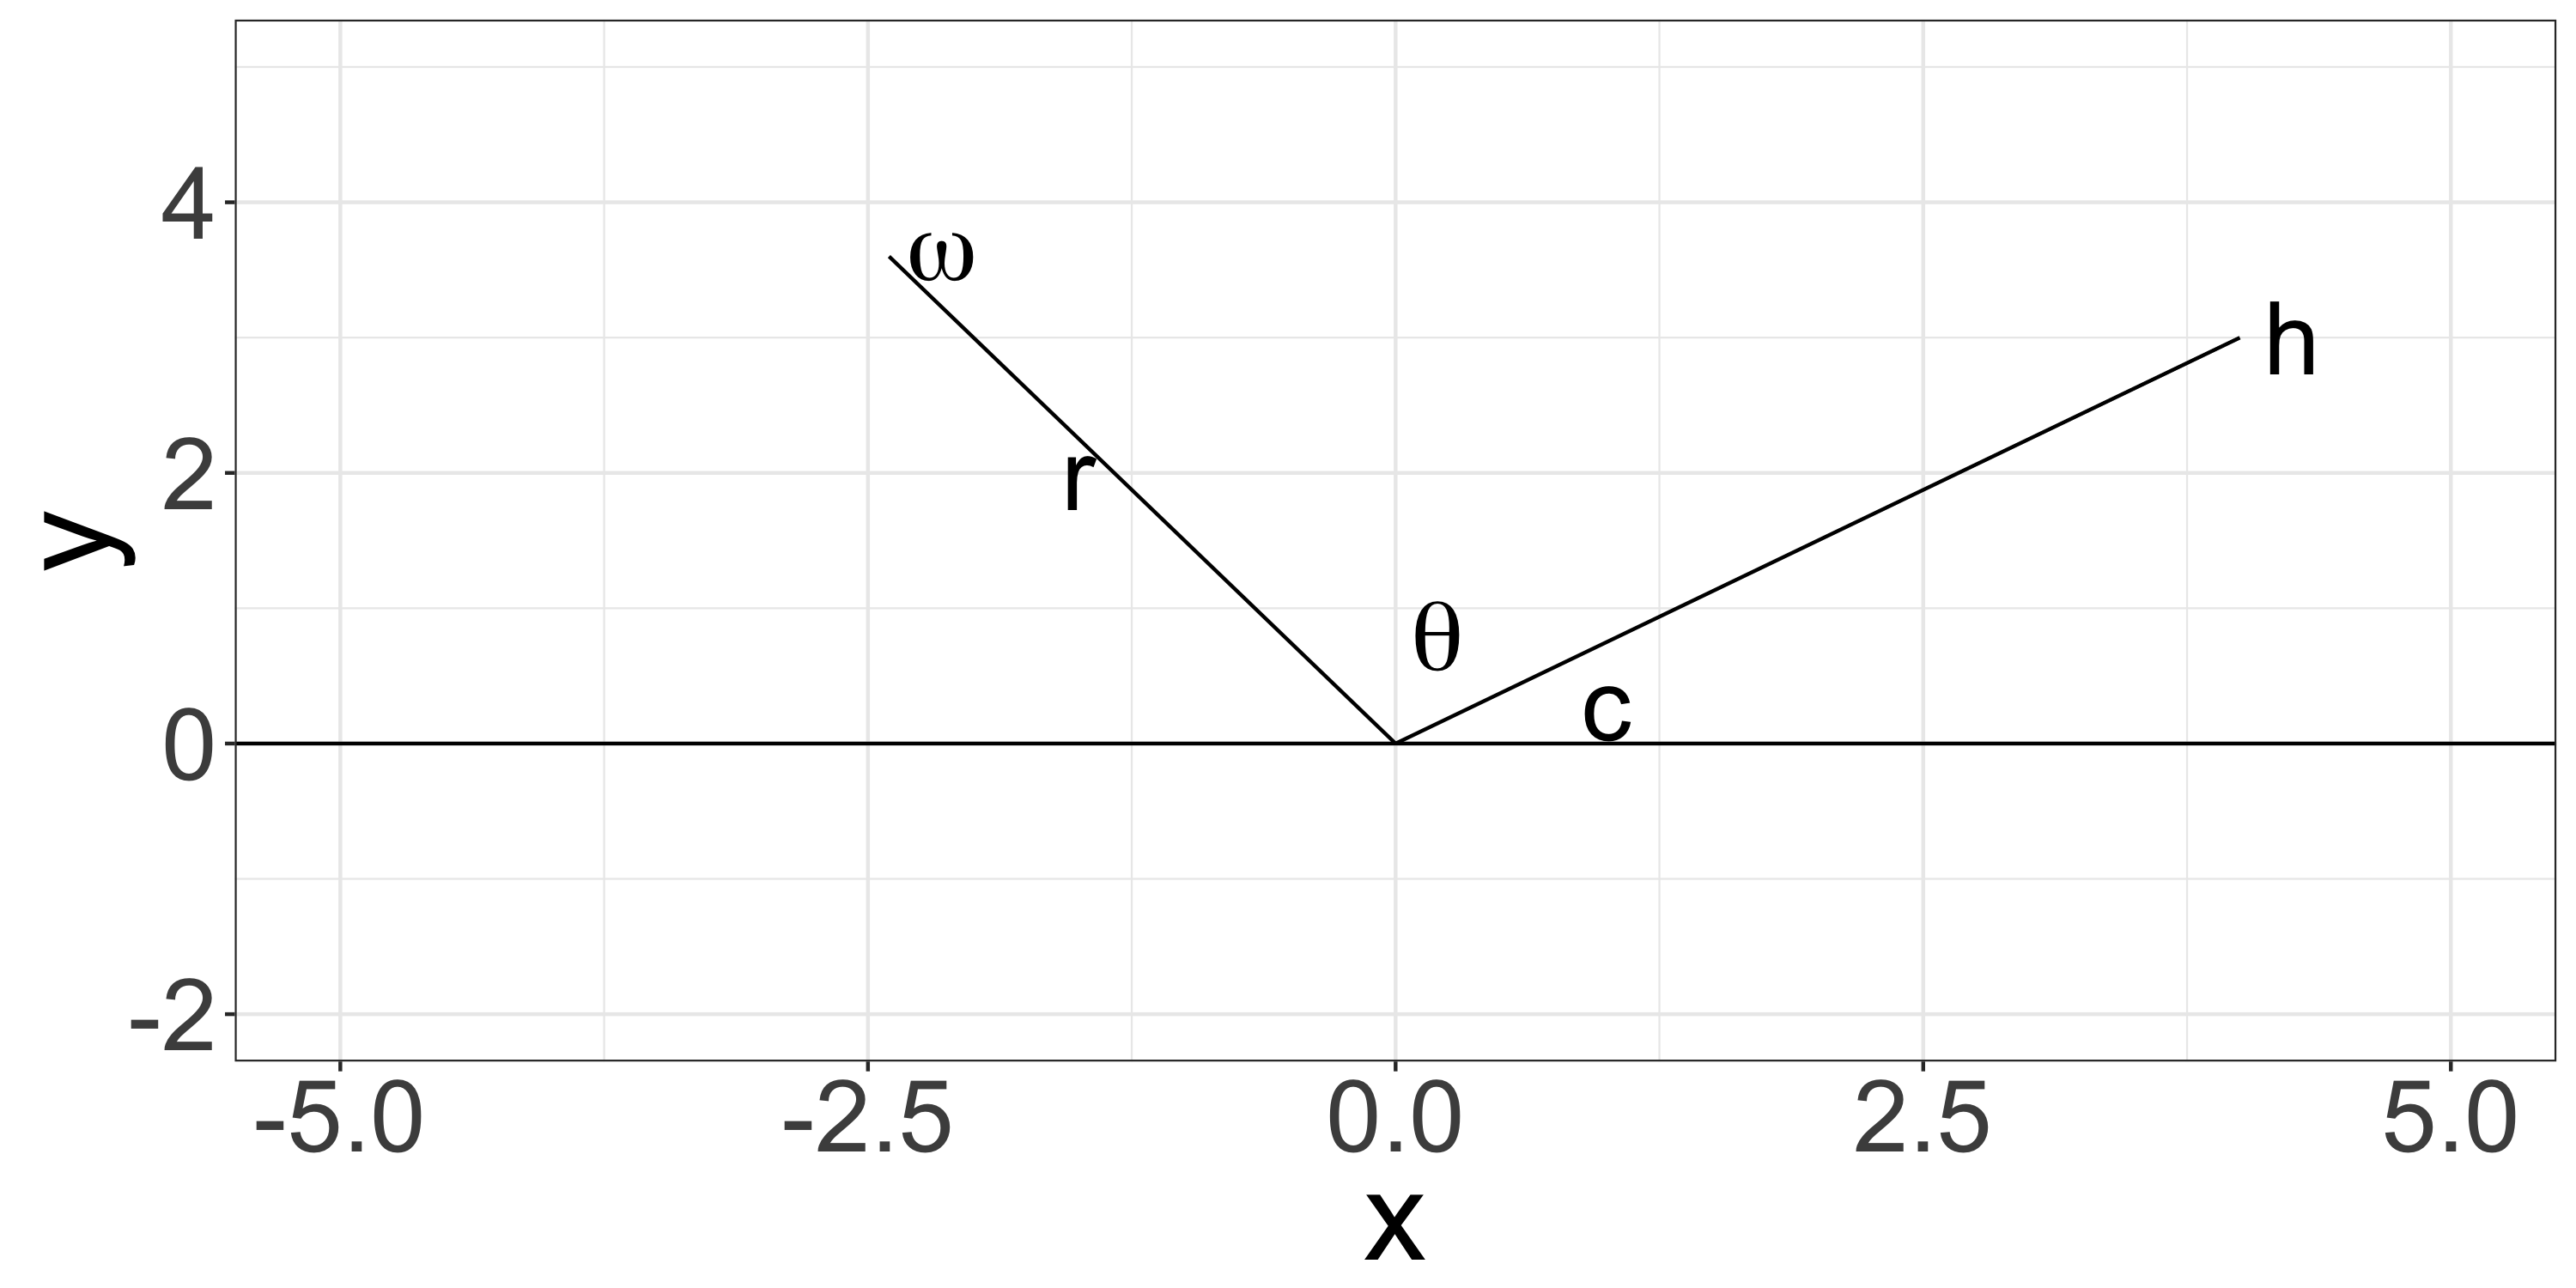
\includegraphics[scale = .1]{angle_plot.png}


%\fbox{ \textbf{Find $\int_{-\pi + c}^{c} \sin(z \cos(\theta)) d\theta$ for $z > 0$ and $c \in (0, \pi)$}} to evaluate the covariance for arbitrary direction in $\mathbb{R}^2$. (an equivalent problem is solving $\int_0^\pi \sin(z\cos(\theta -a)) d\theta$ for each $a \in (0, \pi)$). Mathematica and Wolfram Alpha do not seem to help. We evaluate this integral numerically for different values of $c$, for fixed $z$ shown in the figure below. At $c=\pi/2$ the integral is exactly equal to $\boldsymbol{H}_0(z) \pi$ as evaluated above.
%
% \includegraphics[scale = .35]{integral_one.jpeg}
% \includegraphics[scale = .35]{integral_two.jpeg}
% 
% \includegraphics[scale = .35]{integral_three.jpeg}
% \includegraphics[scale = .35]{integral_five.jpeg}

 By (1.8) on page 24 of \textit{Theory of incomplete cylindrical functions and their applications} by M. M. Agrest  M. S. Maksimov, we have \begin{align*}
 \int_0^{c}  \sin(r\left\lVert \boldsymbol{h}\right\rVert \cos(\theta)) d\theta= \frac{\pi}{2} \boldsymbol{H}_{0}(c, r\left\lVert \boldsymbol{h}\right\rVert)
 \end{align*}where $\boldsymbol{H}_{\nu}(c, z)$ is the incomplete Struve function. Thus, we are left to evaluate \begin{align*} 
 \int_0^\infty \frac{\pi}{2}\left(\boldsymbol{H}_{0}(c, r\left\lVert \boldsymbol{h}\right\rVert) + \boldsymbol{H}_{0}(\pi - c, r\left\lVert \boldsymbol{h}\right\rVert)\right) (1+r^2)^{-\nu-1} r dr
 \end{align*}
 
 \fbox{What is the value of the integral $\int_0^\infty \boldsymbol{H}_{0}(c, r\left\lVert \boldsymbol{h}\right\rVert) (1 +r^2)^{-\nu - 1} r dr$?}
 
 % (5.15) on page 183 of \textit{Theory of incomplete cylindrical functions and their applications} by M. M. Agrest  M. S. Maksimov gives the answer for $\nu = 0$!
 
 
% I propose that  \begin{align*}
% \int_0^\infty  \int_{-\pi - c}^{c} \sin(r\left\lVert \boldsymbol{h}\right\rVert \cos(\theta)) (1 +r^2)^{- \nu - 1} r d\theta dr&= \int_0^\infty \frac{\pi}{2}\left(\boldsymbol{H}_{0}(c, r\left\lVert \boldsymbol{h}\right\rVert) + \boldsymbol{H}_{0}(\pi - c, r\left\lVert \boldsymbol{h}\right\rVert)\right) (1+r^2)^{-\nu-1} r dr \\
% %&= \int_0^\infty \pi\boldsymbol{H}_0(r\left\lVert \boldsymbol{h}\right\rVert)(1 + r^2)^{-\nu - 1} r dr \\
%& =\pi\frac{2^{-\nu -1} \pi \left\lVert \boldsymbol{h}\right\rVert^{\nu}}{\Gamma(\nu+1) \cos(\nu \pi)} \left( \boldsymbol{I}_{\nu }(c, \left\lVert \boldsymbol{h}\right\rVert) - \boldsymbol{L}_{-\nu} (c, \left\lVert \boldsymbol{h}\right\rVert)\right)
%\end{align*}where $\boldsymbol{I}_{\nu }(c, \left\lVert \boldsymbol{h}\right\rVert)$ is the incomplete modified Bessel function and $\boldsymbol{L}_{-\nu} (c, \left\lVert \boldsymbol{h}\right\rVert)$ is the incomplete modified Struve function. Then, when $c = \pi/2$, 

%the above reduces to the answer figured out above, and when $c=\pi$,


%Now, $\mu + \nu = 2$ and $\nu = \nu$ so $\mu = 2- \nu$.

By (5.10) on page 183 of \textit{Theory of incomplete cylindrical functions and their applications} and setting $\mu = 2$ and $\nu = 0$, we have $$\int_0^\infty \frac{-\boldsymbol{H}_{0}(c, ax)}{(x^2 + k^2)^{m+1}}x dx = \frac{\pi}{m!} (-1)^{m+1} \left(\frac{d}{dk^2}\right)^{m}\left\{\frac{I_{0}(c, ak) - \boldsymbol{L}_0(c, ak)}{2}\right\}$$where $I_0(\cdot, \cdot)$ is the incomplete modified Bessel function fo the first kind and $\boldsymbol{L}_0(\cdot, \cdot)$ is the incomplete modified Struve function. When $c=  \pi/2$ these reduce to their \say{complete} versions. This looks close but not exactly right ($m$ is an integer, $\nu$ should be flexible, derivative).



% 
% $\nu = 0$
% $1- \mu  = \nu + 1$
% $\mu = -\nu#
%Furthermore, when $c = \pi/2$, we have \begin{align*}
% \int_0^\infty  \int_{-\pi/2}^{\pi/2} \sin(r\left\lVert \boldsymbol{h}\right\rVert \cos(\theta)) (1 +r^2)^{- \nu - 1} r d\theta dr&= \int_0^\infty \pi\boldsymbol{H}_0(r\left\lVert \boldsymbol{h}\right\rVert)(1 + r^2)^{-\nu - 1} r dr \\
%& =\pi\frac{2^{-\nu -1} \pi \left\lVert \boldsymbol{h}\right\rVert^{\nu}}{\Gamma(\nu+1) \cos(\nu \pi)} \left( \boldsymbol{I}_{\nu }(\left\lVert \boldsymbol{h}\right\rVert) - \boldsymbol{L}_{-\nu} (\left\lVert \boldsymbol{h}\right\rVert)\right)
%\end{align*}
%by 6.814 of I.S. Gradshteyn and I.M. Ryzhik. (compare with Stein for Matern). This gives the nonreversible part in the most nonreversible direction.




%The above example shows us what happens when we are at the ``most nonreversible" part?


 
 
%For the $d$-dimensional case, we follow the argument in Stein (1999) pages 42-43. In particular, note that $$-2M\int_{\vint | \vpla\vint > 0}\sin(\vint^\top \boldsymbol{h})(1 + \vint^\top \vint)^{-\nu- \frac{d}{2}} d\vint$$ only depends on $\vint$ through its length, since for any direction $\boldsymbol{h}$, the above is integrated across all directions of $\vint$. Note that $$\sin(\vint^\top \boldsymbol{h}) = \sin(r |\boldsymbol{h}| \cos(\theta))$$where $\theta$ is the angle between $\vint$ and $\boldsymbol{h}$. Recognizing this and letting $r = \left\lVert \vint \right\rVert$,
%   \begin{align*}
%&\int_{\vint | \vpla \vint > 0}\sin(\vint^\top \boldsymbol{h})(1 + \vint^\top \vint)^{-\nu- \frac{d}{2}} d\vint \\
%&=  \int_{-b}^{\pi - b} \int_0^\infty  \sin(r |\boldsymbol{h}| \cos(\theta))(1 + r^2)^{-\nu-\frac{d}{2}} \sin(\theta)^{d-2} dr d\theta \\
%&=   \int_0^\infty \int_{-b}^{\pi/2 - b}  \sin(r |\boldsymbol{h}| \cos(\theta))(1 + r^2)^{-\nu-\frac{d}{2}} \sin(\theta)^{d-2} d\theta dr \end{align*}
%where $(-b, \pi - b)$ is the values of $\theta$ such that $\vpla \vint > 0$. 
%\begin{align*}
%&= \int_0^\infty \int_0^\pi  \sin(r |\boldsymbol{h}| \cos(\theta))(1 + r^2)^{-\nu-1} \sin(\theta)^{0} dr d\theta \\
%&=2^{-\nu-3/2} |\boldsymbol{h}|^{\nu + 1/2}\sqrt{\pi} \Gamma(-\nu)\left(I_{\nu}(|h|) - L_{-\nu} (|h|)\right)\int_{-a}^{\pi - a} \textrm{sign}(\cos(\theta))|\cos(\theta)|^{\nu +1/2} d\theta 
%%&=-2M \textrm{sign}(h) |h|^{\nu} 2^{-\nu-1} \sqrt{\pi} \Gamma(-\nu + 1/2)\left(I_{\nu}(|h|) - L_{-\nu} (|h|)\right)
% \end{align*}where $a$ is the angle $\boldsymbol{h}$ makes with the hyperplane.
 
 
 
% \section{try Matern}
% 
% We evaluate \begin{align*}
% \int_{\mathbb{R}^d} \cos(\vint^\top \boldsymbol{h}) (1 + \vint^\top \vint)^{-\nu - \frac{d}{2}} d\vint
% \end{align*}
% 
% We follow the argument in Stein 1999 pages 42-43. In particular, note that the above integral only depends on $\vint$ through its length, since for any direction $\boldsymbol{h}$, the above is integrated across all directions of $\vint$. Considering this and noting that \begin{align*}
%\cos(\vint^\top \boldsymbol{h}) = \cos(r \left\lVert \boldsymbol{h}\right\rVert \cos(\theta))
%\end{align*}where $r$ is the length of $\vint$ and $\theta$ is the angle between $\boldsymbol{h}$ and $\vint$, we have 
%\begin{align*}
%\int_0^\pi  \int_0^\infty \cos(r \left\lVert \boldsymbol{h}\right\rVert \cos(\theta)) (1 + r^2)^{-\nu - \frac{d}{2}}  \sin(\theta)^{d-2}  dr d\theta \\ 
%\int_0^\pi K_{\nu} d\theta
%  \end{align*}


 
 
%Considering $r =\pm \left\lVert \vint \right\rVert$ and $\theta = \vint/r$, we have 
%\begin{align*}
%&=\int_0^\infty \int_{S^{d-1}} e^{i r\thet\vpla \boldsymbol{h}}(1 + r^2)^{-\nu- \frac{d}{2}} \left( F(\theta)1_{\{r > 0\}}  - F(\theta)1_{\{r < 0\}}\right) d\theta dr\\
%&=\int_0^\infty \int_{S^{d-1}} (\cos(r\thet\vpla \boldsymbol{h}) + i\sin(r\thet\vpla \boldsymbol{h}))(1 + r^2)^{-\nu- \frac{d}{2}} \left( F(\theta)1_{\{r > 0\}}  - F(\theta)1_{\{r < 0\}}\right) d\theta dr
%\end{align*}




%Also, since $z_{2,1} = z_{1,2}^*$.

%Let $k=2$ for now and let $$C = \begin{pmatrix} C_{11} &  C_{12} \\ C_{21} & C_{22}\end{pmatrix}$$ be the covariance matrix for all of the observations, so that $$\{Y(s_i)\}_{i=1}^n = N(0, C).$$
%
%Taking the maximum likelihood approach and following Kuusela?s approach of using data from a few months for all years, treating observations from different years as independent.


%\section{Future thoughts}
%
%Consider \begin{align*}
%T_{i,j} &= \sum_{k=1}^K Y_{i,k} \phi_k(p_{i,j}) +  \sum_{k=1}^K S_{i,k} \phi_k(p_{i,j})
%\end{align*}where $S_{i,k}$ is the salinity to jointly model the temperature and salinity. This could then be extended to oxygen data and other geochemical data.




%page 24 is the relevant formula for cos cos sin













\end{document}